\chapter{Development} \label{sec:cap3}

This chapter describes the development of the anomaly detection system, which aims to create a toolkit for anomaly detection, model training, and comparison between different models. The toolkit is designed to be modular, allowing for easy integration of new models and features.

\section{System Design}

The anomaly detection system is composed by independent nodes. There is a central node that orchestrates the system, and several nodes that implement the anomaly detection models. Each model node works as a microservice and is responsible for training and predicting anomalies using its own algorithm. The central node is responsible for managing the data flow between the model nodes and the outlier protocol. The system design is shown in \autoref{fig:system-design}.

\begin{figure}[H]
    \centering
    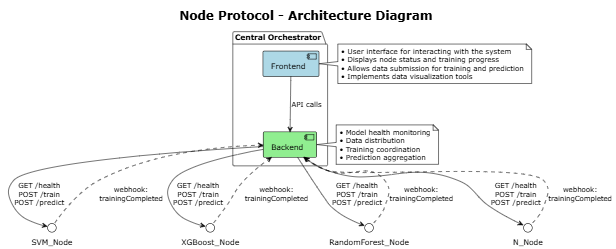
\includegraphics[width=\textwidth]{system-arch.png}
    \caption{Anomaly detection system design}
    \label{fig:system-design}
\end{figure}

\section{Outlier Protocol}

The outlier protocol is a custom protocol based on the OpenAPI specification. It is a simple protocol that describes how the orchestrator interacts with the model nodes, and is based on HTTP messages, which can be grouped into three main categories: \textit{health}, \textit{train}, and \textit{predict}.

\subsection{Health}

Models must implement the \texttt{/health} endpoint. The orchestrator will send a \texttt{get} message at a variable time. If the model does not answer, orchestrator must consider the model as unavailable, and data must not be sent to this model. \autoref{fig:health-message} shows the sequence diagram of the health message and its response. This message also includes the model name, uptime, and last training time.

\begin{figure}[H]
    \centering
    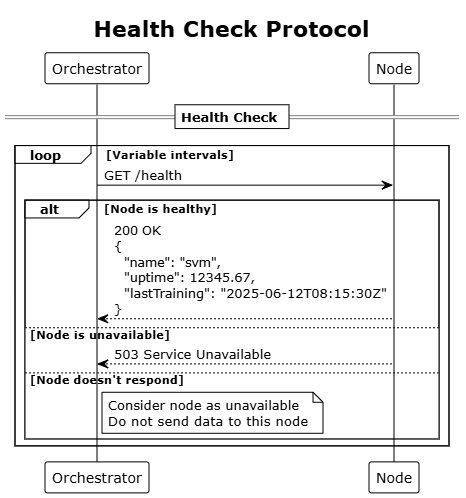
\includegraphics[width=0.75\textwidth]{health.png}
    \caption{Health message sequence diagram}
    \label{fig:health-message}
\end{figure}

\subsection{Train} 

This category describes how models will be trained in order to acquire data for disruption prediction. 

Protocol begins with a \texttt{post} message to the \texttt{/train} model endpoint that contains the number of discharges that will be sent to the models. Models that want to accept the training, answer with a 200 response. Then the orchestrator sends, one by one, the training discharges. After a discharge is received, models must acknowledge it. When all discharges are sent, models shall start the training.

When the training is done, models must inform the orchestrator, as shown in \autoref{fig:train-message}.

\begin{figure}[H]
    \centering
    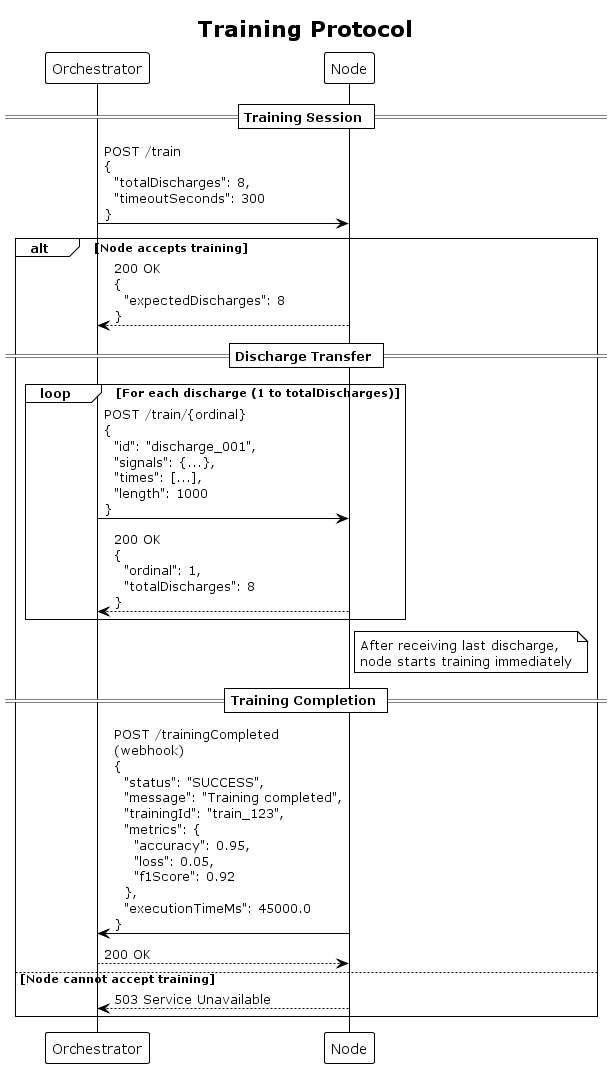
\includegraphics[width=0.75\textwidth]{train.png}
    \caption{Train message sequence diagram}
    \label{fig:train-message}
\end{figure}

\subsection{Predict}
\todo[inline]{Actualizar la figura de predict. En el outlier protocol no están puestas las features que se deben enviar.
\href{https://github.com/outlierClassifier/outlier_protocol/issues/3}{GH issue 3}}
The predict message is sent by the orchestrator to the alive models. It is a \texttt{post} message to the \texttt{/predict} model endpoint.

\missingfigure{Prediction response message sequence diagram}


\section{Outlier Orchestrator}


\section{Outlier Models}

\subsection{\acs{SVM}}

\subsection{XGBoost}

\subsection{CNN-FFT}

\subsection{\acs{OC-SVM}}

\subsection{Isolation Forest}

\subsection{\acs{LSTM}}

